\documentclass[../../../main.tex]{subfiles}

\begin{document}

Whittier College prides itself on doing the right thing.  In Sec. \ref{sec:teaching_philosophy}, I shared my thoughts on physics and the liberal arts.  However, STEM courses are not known for being diverse, nor for fostering equity and inclusion\footnote{This is particularly pronounced for the topic of gender, although explaining the situation is beyond the current scope.}.  What might come as a surprise is that many STEM professors work diligently to foster equity and inclusion in their classes.  In Sec. \ref{sec:oer}, I reflect on open educational resources (OER).  In Sec. \ref{sec:arrange}, I reflect on my flexibility with students.  Finally, in Sec. \ref{sec:cec}, I reflect on our experience with the Artemis program under the Center for Engagement with Communities (CEC).

\subsection{Open Educational Resources (OER)}
\label{sec:oer}

I have helped give three OER workshops with Sonia Chaidez and Azeem Khan on the topic of OER\footnote{I have included my slides for those lectures in the supplemental material.}.  About 1 in 5 students have difficulty buying books.  Students cannot justify spending precious dollars on books when the professor only covers half the content.  Assigning homework from the book forces the students to make hard choices, and we would spend 15-20 hours per week grading.  To address these problems, we use OpenStax resources in all courses for which that is possible\footnote{There is a growing library of texts in areas beyond STEM.  See \url{https://openstax.org} for more information.}.  We have used a homework service called TheExpertTA that administers and grades homework while charging the student \$32.50.  During Spring 2021, my students and I learned to use OpenStax Tutor, the homework system fully integrated with OpenStax textbooks that costs just \$10.00.
\\
\vspace{0.15cm}
OpenStax Tutor is cheap, and the books are free.  Tutor adds several key features beyond TheExpertTA.  First, \textit{reading assignments} can be created to incentivize finishing the reading before class.  Second, the homework problems can be multiple choice, conceptual, or require a longer calculation.  That adds flexibility for our students who may learn differently year to year.  Third, the OpenStax Tutor system uses machine learning to determine the concepts that cause an individual student to struggle.  The system assigns them customized practice problems, and I receive statistical reports on the results.  I use the insights to focus on concepts with which students struggled.  In Fig. \ref{fig:openstax}, the student view of the Tutor assignment planner is shown.  In summary, the system is more adaptable, more feature-rich, and more cost-effective for our students.  Table \ref{tab:oer} contains a list of all courses I have taught, and includes the use of OER.
\\
\vspace{0.15cm}

\begin{figure}
\centering
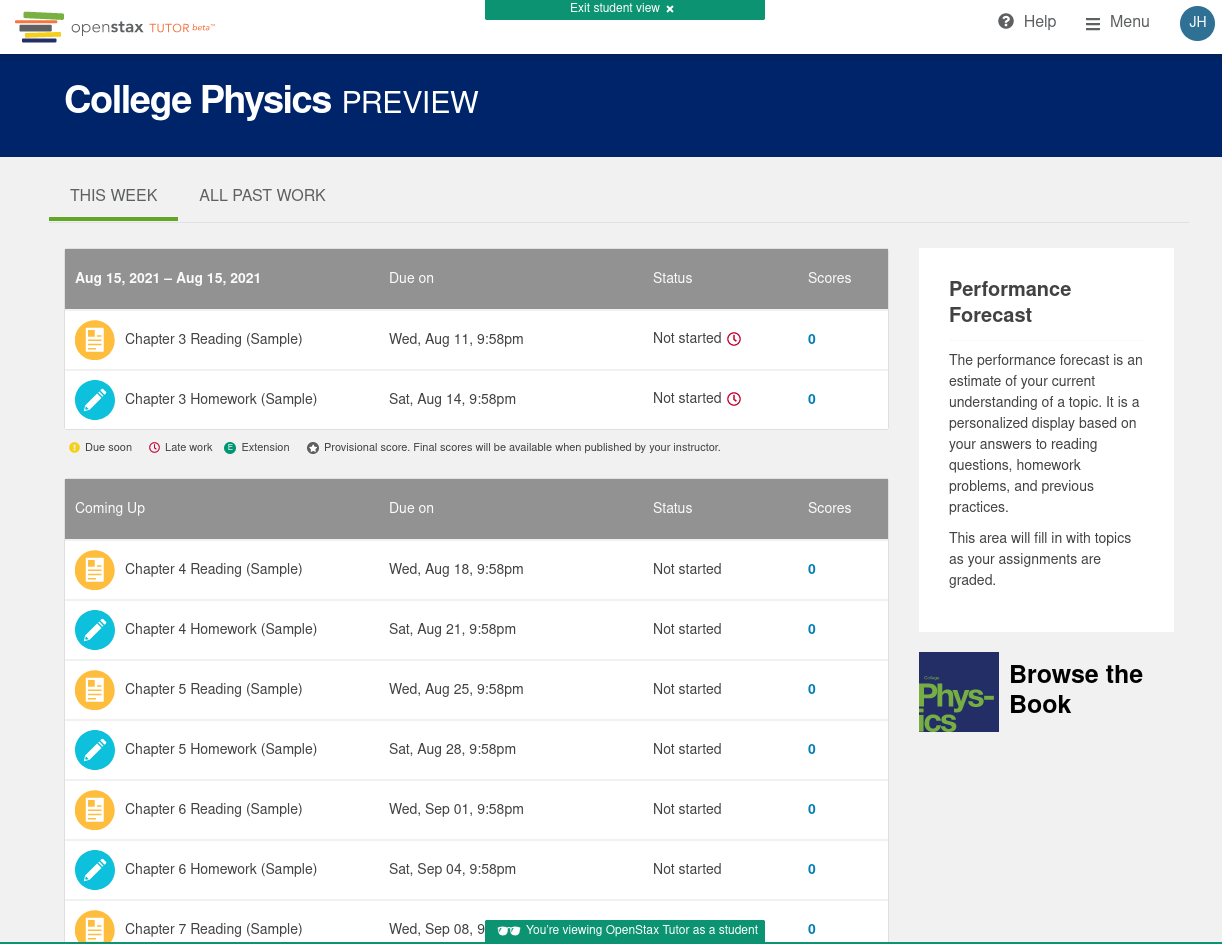
\includegraphics[width=0.4\textwidth]{figures/openstax1.png}
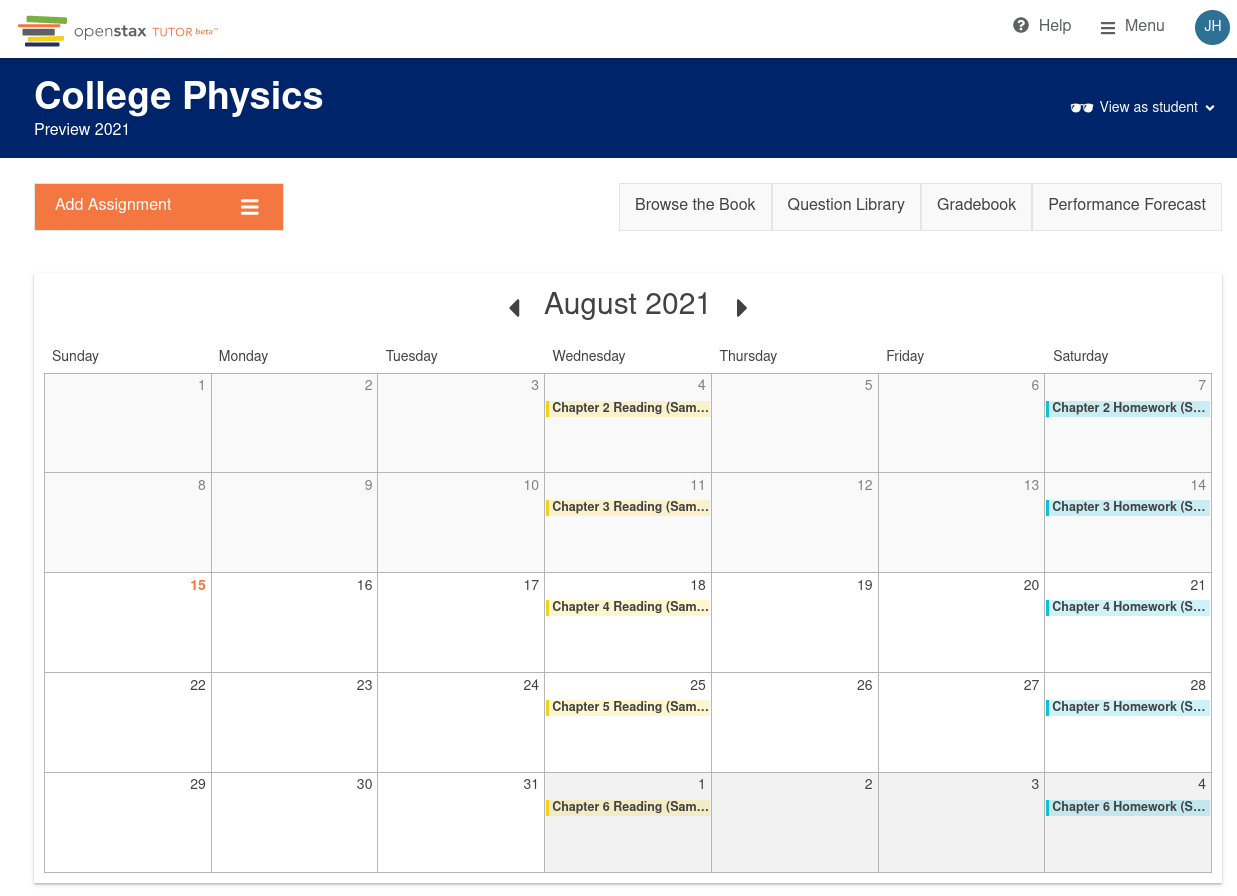
\includegraphics[width=0.4\textwidth]{figures/openstax2.png}
\caption{\label{fig:openstax} (Left) Student view of OpenStax Tutor.  (Right) Professor view.  In both pictures, reading assignments are in yellow and homework assignments are in blue.}
\end{figure}

\begin{table}
\small
\centering
\begin{tabular}{| c | c | c | c | c | c |}
\hline \hline
Semester & Course & Credits & Students & Curriculum feature & OER Usage\\ \hline
Fall 2017 & PHYS135A-01 & 4.0 & 24 & Intro & OpenStax \\ \hline
Fall 2017 & PHYS150-01 & 4.0 & 17 & COM1/Intro & OpenStax \\ \hline
Spring 2018 & PHYS135B-01 & 4.0 & 18 & Intro & OpenStax \\ \hline
Spring 2018 & PHYS180-02 & 5.0 & 19 & COM1/Intro & OpenStax \\ \hline
Spring 2018 & COSC330/PHYS306 & 3.0 & 6 & Advanced & PYNQ-Z1 \\ \hline
Fall 2018 & PHYS135A-01 & 4.0 & 24 & Intro & OpenStax \\ \hline
Fall 2018 & PHYS135A-02 & 4.0 & 26 & Intro & OpenStax \\ \hline
Jan 2019 & COSC390 & 3.0 & 8 & Advanced & open-access text \\ \hline
Spring 2019 & PHYS135B-01 & 4.0 & 25 & Intro & OpenStax \\ \hline
Spring 2019 & PHYS180-02 & 4.0 & 9 & Intro/COM1 & OpenStax \\ \hline
Fall 2019 & PHYS135A-01 & 4.0 & 24 & Intro & OpenStax \\ \hline
Fall 2019 & PHYS150-02/03 & 4.0 & 26 & COM1/Intro & OpenStax \\ \hline
Fall 2019 & INTD255 & 3.0 & 23 & CON2 & OPS \\ \hline
Spring 2020 & COSC330/PHYS306 & 3.0 & 13 & Advanced & PYNQ-Z1 \\ \hline
Spring 2020 & PHYS135B-01 & 4.0 & 23 & Intro & OpenStax \\ \hline
Spring 2020 & PHYS180-02 & 4.0 & 24 & COM1/Intro & OpenStax \\ \hline
Fall 2020 (Module 1) & INTD100-21 & 3.0 & 14 & Intro & -- \\ \hline
Fall 2020 (Module 2) & PHYS330 & 3.0 & 11 & Advanced & -- \\ \hline
Spring 2021 (Module 1) & INTD290 & 3.0 & 26 & CON2,CUL3 & WeVideo \\ \hline
Spring 2021 (Module 2) & PHYS135B-02 & 4.0 & 17 & Intro & OpenStax/Tutor \\ \hline
Spring 2021 (Module 3) & PHYS135B-01 & 4.0 & 25 & Intro & OpenStax/Tutor \\ \hline
-- & Total & 78.0 & -- & -- & -- \\ \hline \hline
Summer 2020 (Session II) & MATH080 & 3.0 & 11 & Intro & OpenStax \\ \hline
\hline
\end{tabular}
\caption{\label{tab:oer} This table is a summary of courses taught in four years, plus Summer sessions.  Not included: PHYS396 (Physics Research for Credit), and PHYS499 (Senior Seminar).  OpenStax and OpenStax Tutor are examples of OER in STEM.  The PYNQ-Z1 is a circuit board integrated with open-source software.  WeVideo is a web-based video editing platform.  OPS stands for Open Polar Server.}
\end{table}

I also use OER in my advanced and liberal arts courses.  In Computer Logic and Digital Circuit Design (COSC330/PHYS306), students design digital electronics on an integrated circuit board called the PYNQ-Z1 by Agilent (\url{https://www.pynq.io}).  Example and project code is all open-source, and our department purchased the boards, so there is zero cost to the student.  In Digital Signal Processing (DSP, now COSC360), the text is open-access.  I write the course software in octave, an open-source language.  In INTD255, the course about Antarctic science, students use the Open Polar Server (OPS) to access data about ice sheets and ice shelves around the world.  In INTD290, the course about Latin American science, students use WeVideo to create digital storytelling projects.  Whittier College has a site license for WeVideo, at no cost to the students.

\subsection{Making Arrangements for a Diverse Group of Students}
\label{sec:arrange}

I have noticed how introductory students struggle to manage time during midterms.  The grading data reveals that most students do well on homework but midterms cause headaches because the students cannot work in groups.  Typically three-fourths of my students are KNS or Biology majors, who are \textit{required} to take algebra-based physics (PHYS135A/B).  They are also required to take courses like organic chemistry.  When midterms in these courses align, students' studying is divided.  I now poll the students regarding the optimal midterm date to maximize study time, and I write take-home exam versions in case a student has to travel on the day the class selects.  The students really appreciate the flexibility.
\\
\vspace{0.15cm}
The flexibility techniques I was learning in 2019-2020 had to be turbo-charged for the module system.  I learned about the Calendly booking service from a workshop.  This taught me what a booking service is, and I located a free version: \url{https://10to8.com}.  The software syncs with my calendar and provides a booking page for the students.  I ensure that my students can grab 30 minutes of my time when they are free.  Sometimes I meet with students when they are on break at work.  Because we use OER, everything is accessible in that moment.
\\
\vspace{0.15cm}
My courses usually involve a student-designed final project.  I have noticed some students create sophisticated projects using our lab equipment, and some create them at home with household items.  I could have jettisoned that part of my syllabus during remote instruction, given that the students had no lab access.  However, the students really shine when designing and executing their own ideas, so I decided it would boost inclusivity by allowing the students to demonstrate DIY projects for each other via Zoom.  Once again, our students rose to the occasion and we all learned.

\subsection{Center for Engagement with Communities: Artemis Program}
\label{sec:cec}

According to a demographic study done by the American Institute of Physics (AIP), women earned about 20\% of bachelor's degrees and doctorates in physics in 2017 \cite{aip}.  Around 3,000 people in the United States enroll in a physics PhD program each year.  Roughly, this means only $\approx 10$ women sign up to earn a PhD in physics \textit{per state, per year.}  I remarked earlier in a footnote that this is a complex issue with many variables not under my control.  However, there are ways in which I can help foster inclusion in STEM.
\\
\vspace{0.15cm}
In Fall 2018, Prof. Serkan Zorba and Samantha Ruiz with the CEC approached me about joining the Artemis Program.  The Artemis Program invites young ladies from local high schools to perform research with Whittier College professors, while CEC staff help them with the Whittier College application.  I served in Spring 2019, and began designing a Python3-based physics education project.  Following my teaching philosphy, I had to establish \textit{order} creatively (Sec. \ref{sec:teaching_philosophy}), and asked the girls to write code together (\textit{shared meaning}).  They presented their results at URSCA 2019, after they wrote Python3 code that gathered data about how quickly and accurately their fellow students solved physics problems.
\\
\vspace{0.15cm}
I served the Artemis Program again in Spring 2020.  Tthe young ladies were to create small, wearable Arduino circuit boards that would relay the location of a lost loved one.  I began with demonstrations and code examples.  The girls got their boards to communicate via WiFi.  Before we could work on making the boards \textit{wearable}, the pandemic struck and URSCA was cancelled.  Nevertheless, the young ladies kept their boards and continued designing at home.  I look forward to seeing some of them again this Fall.

\end{document}
